\documentclass{article}
\usepackage{float}
\usepackage{svg}
\usepackage{amsmath}
\usepackage[utf8]{inputenc}
\usepackage[french]{babel}
\usepackage{graphicx}
\usepackage[T1]{fontenc}
\usepackage{hyperref}
\usepackage{changepage}
\hypersetup{
	colorlinks,
	citecolor=black,
	filecolor=black,
	linkcolor=black,
	urlcolor=black
}
%\graphicspath{ressources/}

\usepackage{blindtext}

\usepackage{subfiles} % Best loaded last in the preamble

\title{Titre}
\author{ }
\date{ }

\begin{document}
\begin{titlepage}
	\begin{center}

		{\Large Université de Mons}\\[1ex]
		{\Large Faculté Des Sciences}\\[1ex]
		{\Large Département d'Informatique}\\[1ex]

		\newcommand{\HRule}{\rule{\linewidth}{0.3mm}}
		% Title
		\HRule \\[0.3cm]
		{ \LARGE \bfseries Projet réseau - Selective-repeat \\[0.3cm]}
		%{ \LARGE \bfseries Rapport d'implémentation  \\[0.1cm]} % Commenter si pas besoin
		\HRule \\[1.5cm]

		% Author and supervisor
		\begin{minipage}[t]{0.45\textwidth}
			\begin{flushleft} \large
				\emph{Professeur:}\\
				Bruno \textsc{Quoitin}\\
				\emph{Assistants:}\\
				Jeremy \textsc{Dubrulle}\\
			\end{flushleft}
		\end{minipage}
		\begin{minipage}[t]{0.45\textwidth}
			\begin{flushright} \large
				\emph{Auteurs:} \\
				Théo \textsc{Godin} 210170 \\
				François \textsc{Vion} 210809 \\
				\emph{Groupe:} \\
				23
			\end{flushright}
		\end{minipage}\\[2ex]

		\vfill

		% Bottom of the page
		\begin{center}
			\begin{tabular}[t]{c c c}
				
\includegraphics[height=1.5cm]{ressources/logoumons.jpg} &
				
\includegraphics[height=1.5cm]{ressources/logofs.jpg} &
			\end{tabular}
		\end{center}~\\

		{\large Année académique 2021-2022}

	\end{center}
\end{titlepage}

\tableofcontents
\newpage

\pagenumbering{arabic}

\section{Construction et exécution}

La compilation du projet se fait en exécutant la commande :
\begin{verbatim}
$ javac reso/examples/selectiverepeat/Demo.java
\end{verbatim}
Et l'exécution : 
\begin{verbatim}
$ java reso.examples.selectiverepeat.Demo [x] [y]
\end{verbatim}
(où x (entier) est le pourcentage de perte de paquets aléatoire et y (entier) le bit rate).\\
Une fois l'exécution terminée les fichiers log et csv sont générés à la racine du projet.

\section{Applications}

Nous avons décidé de suivre l'exemple ping-pong et de créer deux classes application, une qui envoie les données et une autre qui les reçcoit.
L'app sender recoit les données à envoyer en paramètre de son constructeur et passe ensuite ces données à la méthode sendMessage du protocol. 
Tandis que l'app receiver, au lancement de l'application, ne fait qu'écouter.

\section{Selective-repeat}

\subsection{Envoi d'un message}

Un message peut être envoyé par une application via la méthode sendMessage de notre protocol. 
Cette méthode va séparer ce message en plus petits messages de 8 caractères qui vont pouvoir ensuite être envoyés en pipelining.

\subsection{Pipelining}

La méthode pipeliningSend s'occupe d'envoyer des segments tant que la window n'a pas atteint sa taille maximale.

\subsection{Envoi d'un segment}

Afin d'envoyer un segment, la méthode send envoie ce segment à la destination, l'ajoute à l'arrayList représentant la window et finalement crée et démarre un timer afin de gérer les timeout pour ce segment.\\
Du côté du receveur, la méthode sendAck permet d'envoyer un acquittement de même sequence number que le segment reçu.

\subsection{Timeout et RTO}

Si un timer arrive à sa fin, le segment associé est ré-envoyé et un nouveau timer est créé. 
La durée du timer est calculée de la même manière que vue au cours.
Si l'on a un timeout, la durée de celui ci est doublée et si l'envoyeur reçoit un ACK, les valeurs pour R, SRTT, devRTT et RTO (durée du timer) sont recalculées avec les formules indiquées dans le cours.

\subsection{Réception d'un acquittement}

Lors de la réception d'un acquittement par l'envoyeur, si le segment correspondant est présent dans la window, celui-ci est marqué comme acquitté.
Ainsi, au prochain appel de la méhtode verifyWindow, la fenêtre sera avancée pour chaque paquets ayant reçu sont acquittement. 

\section{Contrôle de congestion}

Afin de gérer le contrôle de congestion, la taille de la fenêtre est modifié au cours du processus afin d'avoir une taille optimale tout au long de l'envoi.
Cela se fait lorsque l'envoyeur reçoit un ACK ou lors d'un timeout.
Lors de la réception d'un ACK, on double la taille de la fenêtre si celle-ci est inférieure au sstresh (fixé à 100 au départ). Si elle est inférieure, on l'incrémente de 1.
Lors d'un timeout, la taille de fenêtre est fixée à 1 et le sstresh est fixé à la moitié de la dernière valeur de fenêtre. Dans le cas où la fenêtre avait une taille de 1, le sstresh est fixé à 1.\\
Voici un graphique qui montre l'évolution de la taille de la fenêtre au fil du processus d'envoi avec une perte de paquet de 20\%. \\
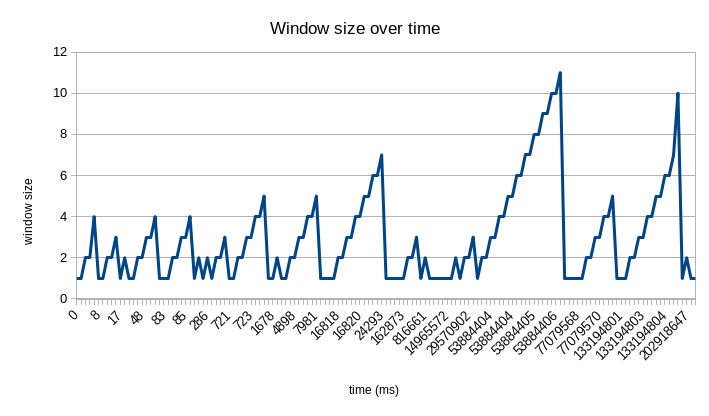
\includegraphics[height=7cm]{ressources/windowChart.png}



\section{Bugs rencontrés}

Nous avons remarqués grâce aux logs que le receveur recevait des paquets acquittés. 
Après avoir testé chaque méthode envoyant des messages, la source du bug n'a toujours pas été découverte car aucune d'entre elles n'envoie de message acquitté. 
Ce bug a donc été contourné en ajoutant au protocol l'attribut actor permettant de savoir si l'application courrante est l'envoyeur ou le receveur, ce qui est testé lors de la réception d'un message.\\

Malgré avoir suivi la méthode et les calculs de RTO indiqués dans le cours, nous avons pu voir que celui-ci croit beaucoup trop pendant le processus, ce qui mène à un temps de processus disproportionné. Nous n'avons pas su déterminer l'origine de ce problème.\\

La taille de la fenêtre étant recalculée à chaque ACK reçu, le graphique possède une croissance en escalier car car il y a un délai avant que le prochain ACK arrive. 

\section{Outils}

Notre projet comporte un système de logs implémenté dans la classe Tools.
La méthode log nécessite 3 paramètres : 
\begin{enumerate}
\item le temps
\item l'acteur
\item l'action
\end{enumerate}
Ces 3 informations sont ensuite enregistrées dans le fichier selectiverepeat.log à la racine du projet.\\
Nous avons également implémenté la méthode plot afin de suivre l'évolution de la fenêtre.
Cette méthode permet de générer un fichier csv contenant les données de l'évolution de la fenêtre en fonction du temps. 

\end{document}
